\begin{figure*}[htbp]
    \centering
    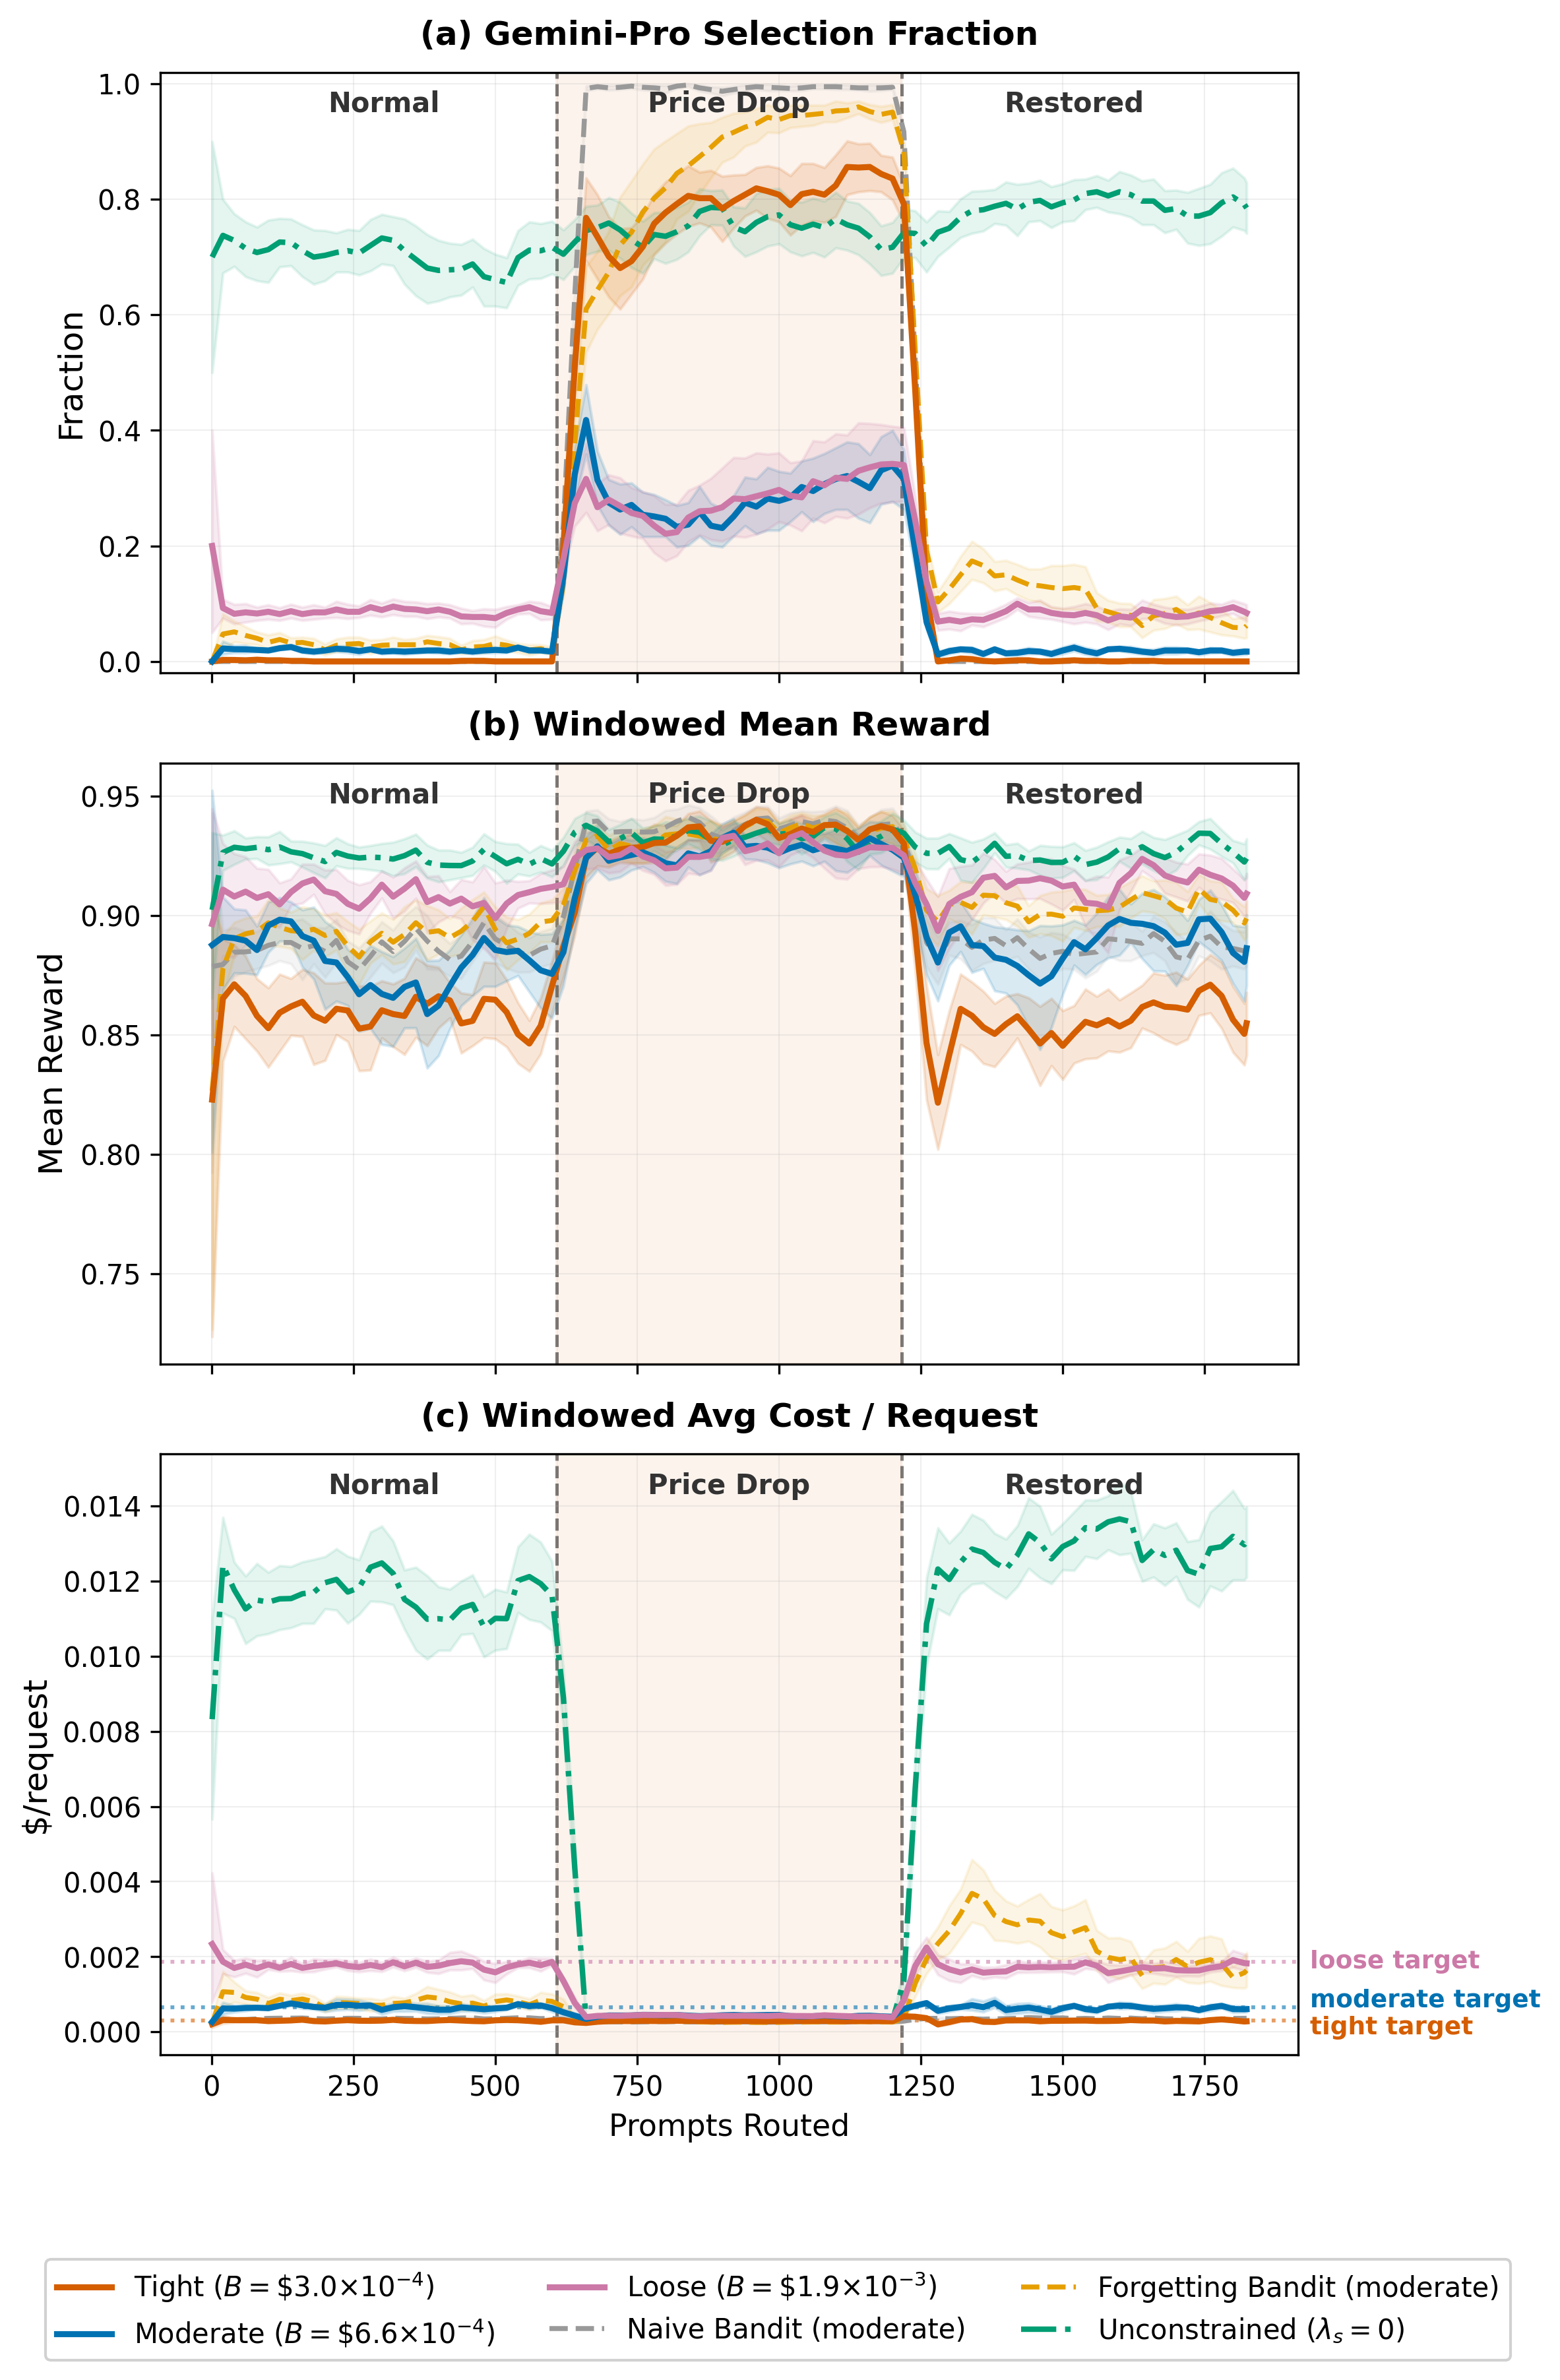
\includegraphics[width=\linewidth]{../experiments/02_budget_plus_drift/results/adaptation_dynamics.pdf}
    \caption{Adaptation dynamics under cost drift: normal pricing
    $\to$ Gemini price drop (step~609) $\to$ price restored
    (step~1217).
    $K{=}3$, 20~seeds, 95\% bootstrap CI.
    Solid coloured lines show ParetoBandit at three budget levels;
    dashed grey and orange show the Naive Bandit and Forgetting
    Bandit at moderate budget; dash-dot green is unconstrained.
    %
    \textbf{(a)}~Gemini-Pro selection fraction: ParetoBandit
    surges in Phase~2 (tight reaches ${\sim}72\%$) and returns to
    near-zero in Phase~3.  The Forgetting Bandit (orange) shifts
    to Gemini faster than the Naive Bandit (grey) because
    forgetting down-weights stale Phase~1 observations, but
    neither has cost control.
    %
    \textbf{(b)}~Windowed mean reward: all conditions benefit
    from cheap Gemini in Phase~2.  The Forgetting Bandit
    achieves higher Phase~2 reward than ParetoBandit because it
    adopts Gemini more aggressively---but panel~(c) reveals the
    cost.
    %
    \textbf{(c)}~Windowed average cost per request; dotted lines
    mark budget targets.  ParetoBandit hugs the target in all
    three phases.  The Forgetting Bandit overshoots from Phase~1
    onward; the Naive Bandit overshoots in Phase~3 when it cannot
    revert from its Gemini-heavy Phase~2 policy.
    See Table~\ref{tab:budget_compliance} for full compliance
    comparisons across all five conditions.
    }
    \label{fig:exp02_adaptation}
\end{figure*}
